% Exam Template for UMTYMP and Math Department courses
%
% Using Philip Hirschhorn's exam.cls: http://www-math.mit.edu/~psh/#ExamCls
%
% run pdflatex on a finished exam at least three times to do the grading table on front page.
%
%%%%%%%%%%%%%%%%%%%%%%%%%%%%%%%%%%%%%%%%%%%%%%%%%%%%%%%%%%%%%%%%%%%%%%%%%%%%%%%%%%%%%%%%%%%%%%

% These lines can probably stay unchanged, although you can remove the last
% two packages if you're not making pictures with tikz.
\documentclass[11pt]{exam}
\RequirePackage{amssymb, amsfonts, amsmath, latexsym, verbatim, xspace, setspace, graphicx, caption}


% By default LaTeX uses large margins.  This doesn't work well on exams; problems
% end up in the "middle" of the page, reducing the amount of space for students
% to work on them.
\usepackage[margin=1in]{geometry}
\usepackage[english]{babel}
\usepackage[autostyle]{csquotes} %%%% This package allows Tex to recognize quotation marks with the \enquote command. 


% Here's where you edit the Class, Exam, Date, etc.
\newcommand{\class}{MAT 303}
\newcommand{\term}{Summer II 2018}
\newcommand{\examnum}{Midterm}
\newcommand{\examdate}{07/26/18}
\newcommand{\timelimit}{3 hours and 25 minutes}

% For an exam, single spacing is most appropriate
\singlespacing
% \onehalfspacing
% \doublespacing

% For an exam, we generally want to turn off paragraph indentation
\parindent 0ex
\title{MAT 303 - Summer II 2018: Midterm}
\begin{document} 

% These commands set up the running header on the top of the exam pages
\pagestyle{head}
\firstpageheader{}{}{}\textbf{}
\runningheader{\class}{\examnum\ - Page \thepage\ of \numpages}{\examdate}
\runningheadrule

\begin{flushright}
\begin{tabular}{p{2.8in} r l}
\textbf{\class} & \textbf{Name (Print):} & \makebox[2in]{\hrulefill}\\
\textbf{\term} &&\\
\textbf{\examnum} &&\\
\textbf{\examdate} &&\\
\textbf{Time Limit: \timelimit} & ID number & \makebox[2in]{\hrulefill}
\end{tabular}\\
\end{flushright}
\rule[1ex]{\textwidth}{.1pt}

\begin{center}
\large{\textbf{Instructions}}
\end{center}

\begin{minipage}[t]{3.7in}
\vspace{0pt}
\begin{itemize}

\item This exam contains \numpages\ pages (including this cover page) and
\numquestions\ problems.  Check to see if any pages are missing.  Enter
all requested information on the top of this page, and put your initials
on the top of every page, in case the pages become separated.

\item You may \textit{not} use your books, notes, or any device that is capable of accessing the internet on this exam (e.g., smartphones, smartwatches, tablets). You may not use a calculator.

\item \textbf{Organize your work}, in a reasonably neat and coherent way, in
the space provided. Work scattered all over the page without a clear ordering will 
receive very little credit.  

\item \textbf{Mysterious or unsupported answers will not receive full
credit}.

\end{itemize}

\end{minipage}
\hfill
\begin{minipage}[t]{2.3in}
\vspace{0pt}
%\cellwidth{3em}
\gradetablestretch{2}
\vqword{Problem}
\addpoints % required here by exam.cls, even though questions haven't started yet.	
\gradetable[v]%[pages]  % Use [pages] to have grading table by page instead of question

\end{minipage}
\newpage % End of cover page

%%%%%%%%%%%%%%%%%%%%%%%%%%%%%%%%%%%%%%%%%%%%%%%%%%%%%%%%%%%%%%%%%%%%%%%%%%%%%%%%%%%%%
%
% See http://www-math.mit.edu/~psh/#ExamCls for full documentation, but the questions
% below give an idea of how to write questions [with parts] and have the points
% tracked automatically on the cover page.
%
%
%%%%%%%%%%%%%%%%%%%%%%%%%%%%%%%%%%%%%%%%%%%%%%%%%%%%%%%%%%%%%%%%%%%%%%%%%%%%%%%%%%%%%

\begin{questions}

% Basic question
%%%%%%%%%%%%%%

\addpoints
\question Find the general solution to each of the following first-order differential equations. Note: solutions can be written implicitely, or depend on the computation of certain integrals which can't be expressed in terms of elementary functions. Primes denote derivatives relative to the independent variable $t$. 
\begin{parts}
\part[5] 
\begin{equation*}
(t^2+1)x'+ 2tx = t
\end{equation*}
\vfill
\part[5] 
\begin{equation*}
2txx'=t^2 + x^2
\end{equation*}
\vfill
\newpage
\part[10] 
\begin{equation*}
3t^2+x^2 + (4tx+6x^2)x' = 0
\end{equation*}
\vfill
\end{parts}

\newpage 

%%%%%%%%%%%%%%%%%%%%%%%%%%%%%%%%%%%
\addpoints 
\question Match the differential equations and slope fields below. Explain your reasoning in the space provided below each equation.   

\begin{figure}[h]
\centering
\begin{minipage}{.5\textwidth}
  \centering
  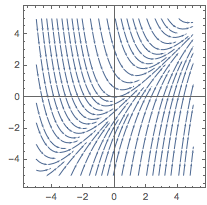
\includegraphics[width=.4\linewidth]{slopefield1}
  \caption{Slope field 1}
  %\label{fig:test1}
\end{minipage}%
\begin{minipage}{.5\textwidth}
  \centering
  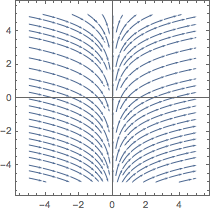
\includegraphics[width=.4\linewidth]{slopefield2}
  \caption{Slope field 2}
 %\label{fig:test2}
\end{minipage}
\end{figure}

\begin{figure}[h]
\centering
\begin{minipage}{.5\textwidth}
  \centering
  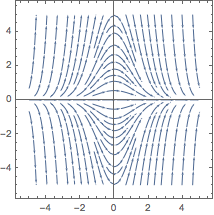
\includegraphics[width=.4\linewidth]{slopefield3}
  \caption{Slope field 3}
  %\label{fig:test3}
\end{minipage}%
\begin{minipage}{.5\textwidth}
  \centering
  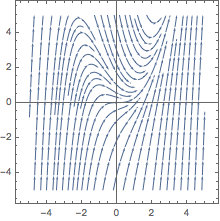
\includegraphics[width=.4\linewidth]{slopefield4}
  \caption{Slope field 4}
 %\label{fig:test4}
\end{minipage}
\end{figure}

\begin{parts}
\part[5] 
\begin{equation*}
y'=-xy
\end{equation*} 
\vfill
\part[5] 
\begin{equation*}
y'=\frac{1}{x} 
\end{equation*}
\vfill
\newpage
\part[5]  
\begin{equation*}
y'= x-y
\end{equation*}
\vfill
\part[5] 
\begin{equation*}
y'=x^2-y
\end{equation*}
\vfill
\end{parts}

\newpage

%%%%%%%%%%%%%%%%%
\addpoints
\question A certain logistic population naturally satisfies the equation
\begin{equation*}
\frac{dP}{dt} = 4P - P^2.
\end{equation*}
Answer the following questions about this populational model:

\begin{parts}
\part[2] What are the values of the equilibrium solutions? Classify each of them into stable, semistable or unstable. 
\vfill
\part[3] What is the value of initial population which yields maximal initial populational growth (i.e., maximizes $P'(0)$)?
\vfill
\part[5] If the population is to be harvarsted at a constant rate $h >0$, what is the new differential equation modelling this phenomenon?
\vfill
\newpage
\part[4] Regarding the equation you found in part (c), how does the number of equilibrium solutions vary in terms of $h$? 
\vfill
\part[4] How does the stability classification vary in terms of $h$?
\vfill
\part[2] Sketch the bifurcation diagram for the equation from part (c). 
\vfill
\end{parts}
\newpage
%%%%%%%%%%%%%%%%%

\addpoints

\addpoints
\question Find general solutions to the following higher-order linear differential equations:

\begin{parts}
\part[5] 
\begin{equation*}
x^{(3)} + x -10 = 0
\end{equation*}
\vfill
\part[5] 
\begin{equation*}
x^{(3)} + 4x'' + 5x' +2x = 0
\end{equation*}
\vfill
\newpage
\part[5] 
\begin{equation*}
x^{(4)} -4x = 0
\end{equation*}
\vfill
\part[5]
\begin{equation*}
x^{(4)} + 2x'' + x = 0
\end{equation*}
\vfill
\end{parts}
\newpage

%%%%%%%%%%%%%%%%%%%%
\addpoints
\question Consider the initial-value problem
\begin{align*}
y' & = x+y, \\
y(0) & = 1.
\end{align*}


\begin{parts}
\part[10]  Estimate the value of $y(1)$ using Euler's method with $3$ steps.  
\vfill 
\newpage 
\part[10] Estimate the value of $y(1)$ using the 3rd order Picard approximation. 
\vfill
\end{parts}

%%%%%%%%%%%%%%%%%%%%%%%%%%

\end{questions}
\end{document}